\documentclass[12pt, a4paper]{article}
\usepackage[slovene]{babel}
\usepackage[utf8]{inputenc}
\usepackage[T1]{fontenc}
\usepackage{amsmath, amssymb, fullpage, graphicx}

\begin{document}

\section{Uvod}

Pri tej nalogi smo imeli nekaj dela s teorijo grafov. Natan\v{c}neje, opravka smo imeli z obojestransko povezanimi
grafi. Z njimi lahko namre\v{c} natan\v{c}neje obravnavamo populacijske modele, saj so taki grafi lokalizirani.

Modeliramo lahko na primer prena\v{s}anje vica/ideje/bolezni preko populacije. Povezave med ljudmi v taki populaciji so
stohasti\v{c}ne.

Poleg tega je bilo potrebno \v{s}e preveriti Kapitzov populacijski model. Kot pi\v{s}e v navodilu je pri\v{c}el s
preprostimi predpostavkami in pri\v{s}el do zanimivih rezultatov. To bomo obravnavali v nalogah 2 in 3.

\section{Povezave}

V tej nalogi smo pri\v celi z grafom, kjer je bilo vsako vozli\v s\v ce povezano zgolj z najblji\v zjimi sosedi. To
\v stevilo mora biti sodo, saj bi v nasprotnem primeru dobili orientirane grafe. Prav tako moramo predpostaviti, da je
vsako vozli\v s\v ce povezano samo s seboj. Tako lahko s potenciranjem matrike povezav pridemo do premera grafa.

Tak graf seveda ni realen -- da dobimo populacijo, ki nas bolje opi\v se moramo povezave stohasti\v cno premikati
znotraj matrike povezav. Ta je simetri\v cna, ima zgolj enice in ni\v cle. Indeksi stolpcev predstavljajo vozli\v s\v ca,
indeksi vrstic pa predstavljajo vozli\v s\v ce, na katerega je stolpec povezan.

Ker poznamo \v stevilo povezav $D$, ki je majhno v primerjavi s \v stevilom vozli\v s\v c, je veliko prostora za
optimizacijo. Sam sem na primer vse povezave pospravil v lo\v ceno tabelo, naklju\v cno \v stevilo, pa je predstavljalo
indeks povezave. S tem se izognemo nepotrebnem \v zrebanju \v stevil. Dobljeno enico v matriki pobri\v semo in prestavimo
na novo mesto. Tu je spet prostor za optimizacijo: enic je veliko manj kot ni\v cel, zato se teh ne spla\v ca imeti
pospravljenih v lo\v ceni tabeli. Zato sem najprej preveril, \v ce je verjetnost, da iz\v zrebamo ni\v clo ve\v cja od
0.5. \v Ce je, potem lahko \v zrebamo, sicer pa jo enostavno premikako po sosedih, dokler ne pridemo do nje in jo
pretvorimo v enico.

To po\v cnemo, dokler so izpolnjeni vsi izmed slede\v cih pogojev:
\begin{itemize}
	\item[(a)]{\v stevilo iteracij manj\v se od $10^4$,}
	\item[(b)]{koeficient gru\v cavosti je ve\v cji od $0.001$,}
	\item[(c)]{gru\v cavost se je zadnjih $100$ iteracij spremenila za ve\v c kot $0.001$.}
\end{itemize}

V kolikor je eden izmed teh pogojev neizpolnjen je se iteracijo prekine. Zadnji pogoj sem imel sprva nastavljen na
vsakih 500 iteracij, vendar je na vsakih 100 zadosten pogoj.

\begin{figure}[H]\centering
	% GNUPLOT: LaTeX picture with Postscript
\begingroup
  \makeatletter
  \providecommand\color[2][]{%
    \GenericError{(gnuplot) \space\space\space\@spaces}{%
      Package color not loaded in conjunction with
      terminal option `colourtext'%
    }{See the gnuplot documentation for explanation.%
    }{Either use 'blacktext' in gnuplot or load the package
      color.sty in LaTeX.}%
    \renewcommand\color[2][]{}%
  }%
  \providecommand\includegraphics[2][]{%
    \GenericError{(gnuplot) \space\space\space\@spaces}{%
      Package graphicx or graphics not loaded%
    }{See the gnuplot documentation for explanation.%
    }{The gnuplot epslatex terminal needs graphicx.sty or graphics.sty.}%
    \renewcommand\includegraphics[2][]{}%
  }%
  \providecommand\rotatebox[2]{#2}%
  \@ifundefined{ifGPcolor}{%
    \newif\ifGPcolor
    \GPcolortrue
  }{}%
  \@ifundefined{ifGPblacktext}{%
    \newif\ifGPblacktext
    \GPblacktexttrue
  }{}%
  % define a \g@addto@macro without @ in the name:
  \let\gplgaddtomacro\g@addto@macro
  % define empty templates for all commands taking text:
  \gdef\gplbacktext{}%
  \gdef\gplfronttext{}%
  \makeatother
  \ifGPblacktext
    % no textcolor at all
    \def\colorrgb#1{}%
    \def\colorgray#1{}%
  \else
    % gray or color?
    \ifGPcolor
      \def\colorrgb#1{\color[rgb]{#1}}%
      \def\colorgray#1{\color[gray]{#1}}%
      \expandafter\def\csname LTw\endcsname{\color{white}}%
      \expandafter\def\csname LTb\endcsname{\color{black}}%
      \expandafter\def\csname LTa\endcsname{\color{black}}%
      \expandafter\def\csname LT0\endcsname{\color[rgb]{1,0,0}}%
      \expandafter\def\csname LT1\endcsname{\color[rgb]{0,1,0}}%
      \expandafter\def\csname LT2\endcsname{\color[rgb]{0,0,1}}%
      \expandafter\def\csname LT3\endcsname{\color[rgb]{1,0,1}}%
      \expandafter\def\csname LT4\endcsname{\color[rgb]{0,1,1}}%
      \expandafter\def\csname LT5\endcsname{\color[rgb]{1,1,0}}%
      \expandafter\def\csname LT6\endcsname{\color[rgb]{0,0,0}}%
      \expandafter\def\csname LT7\endcsname{\color[rgb]{1,0.3,0}}%
      \expandafter\def\csname LT8\endcsname{\color[rgb]{0.5,0.5,0.5}}%
    \else
      % gray
      \def\colorrgb#1{\color{black}}%
      \def\colorgray#1{\color[gray]{#1}}%
      \expandafter\def\csname LTw\endcsname{\color{white}}%
      \expandafter\def\csname LTb\endcsname{\color{black}}%
      \expandafter\def\csname LTa\endcsname{\color{black}}%
      \expandafter\def\csname LT0\endcsname{\color{black}}%
      \expandafter\def\csname LT1\endcsname{\color{black}}%
      \expandafter\def\csname LT2\endcsname{\color{black}}%
      \expandafter\def\csname LT3\endcsname{\color{black}}%
      \expandafter\def\csname LT4\endcsname{\color{black}}%
      \expandafter\def\csname LT5\endcsname{\color{black}}%
      \expandafter\def\csname LT6\endcsname{\color{black}}%
      \expandafter\def\csname LT7\endcsname{\color{black}}%
      \expandafter\def\csname LT8\endcsname{\color{black}}%
    \fi
  \fi
  \setlength{\unitlength}{0.0500bp}%
  \begin{picture}(7200.00,5040.00)%
    \gplgaddtomacro\gplbacktext{%
      \csname LTb\endcsname%
      \put(682,704){\makebox(0,0)[r]{\strut{} 0}}%
      \put(682,1411){\makebox(0,0)[r]{\strut{} 1}}%
      \put(682,2117){\makebox(0,0)[r]{\strut{} 2}}%
      \put(682,2824){\makebox(0,0)[r]{\strut{} 3}}%
      \put(682,3531){\makebox(0,0)[r]{\strut{} 4}}%
      \put(682,4238){\makebox(0,0)[r]{\strut{} 5}}%
      \put(814,484){\makebox(0,0){\strut{} 0}}%
      \put(1436,484){\makebox(0,0){\strut{} 200}}%
      \put(2058,484){\makebox(0,0){\strut{} 400}}%
      \put(2680,484){\makebox(0,0){\strut{} 600}}%
      \put(3303,484){\makebox(0,0){\strut{} 800}}%
      \put(3925,484){\makebox(0,0){\strut{} 1000}}%
      \put(4547,484){\makebox(0,0){\strut{} 1200}}%
      \put(5169,484){\makebox(0,0){\strut{} 1400}}%
      \put(5791,484){\makebox(0,0){\strut{} 1600}}%
      \put(5923,704){\makebox(0,0)[l]{\strut{} 0}}%
      \put(5923,1439){\makebox(0,0)[l]{\strut{} 0.1}}%
      \put(5923,2174){\makebox(0,0)[l]{\strut{} 0.2}}%
      \put(5923,2909){\makebox(0,0)[l]{\strut{} 0.3}}%
      \put(5923,3644){\makebox(0,0)[l]{\strut{} 0.4}}%
      \put(5923,4379){\makebox(0,0)[l]{\strut{} 0.5}}%
      \put(176,2541){\rotatebox{-270}{\makebox(0,0){\strut{}Premer grafa -- $d$}}}%
      \put(6692,2541){\rotatebox{-270}{\makebox(0,0){\strut{}Koeficient gru\v{c}avosti -- $c$}}}%
      \put(3302,154){\makebox(0,0){\strut{}Indeks iteracije -- $i$}}%
      \put(3302,4709){\makebox(0,0){\strut{}$N = 100$, $D = 20$}}%
    }%
    \gplgaddtomacro\gplfronttext{%
      \csname LTb\endcsname%
      \put(4804,4206){\makebox(0,0)[r]{\strut{}$d$}}%
      \csname LTb\endcsname%
      \put(4804,3986){\makebox(0,0)[r]{\strut{}$c$}}%
    }%
    \gplbacktext
    \put(0,0){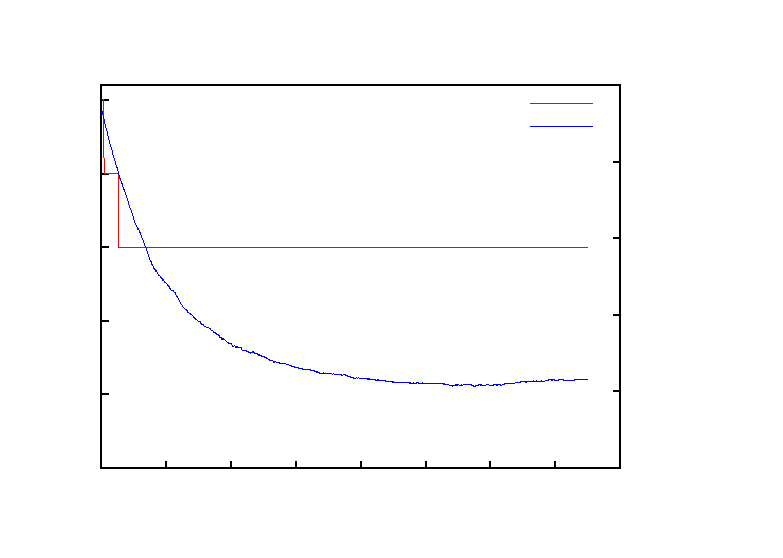
\includegraphics{graph-100-20}}%
    \gplfronttext
  \end{picture}%
\endgroup

	\caption{Za primerjavo lahko vidimo kako se s \v stevilom iteracij spreminjata koeficient gru\v cavosti
		ter premer grafa.}
\end{figure}

\end{document}
